\documentclass[12pt,journal,compsoc]{IEEEtran}

\usepackage{graphicx}
\usepackage{caption}

\ifCLASSOPTIONcompsoc
\else
\fi
\ifCLASSINFOpdf

\else

\fi

\newcommand\MYhyperrefoptions{bookmarks=true,bookmarksnumbered=true,
pdfpagemode={UseOutlines},plainpages=false,pdfpagelabels=true,
colorlinks=true,linkcolor={black},citecolor={black},urlcolor={black},
pdftitle={Ceng435 - Term Project 2},
pdfsubject={Ceng435 - Term Project 2},
pdfauthor={Koray Can Yurtseven, Aykut Yardim},
pdfkeywords={Network, LaTeX, paper, template}}

\begin{document}

\title{Data Communications and Networking \\ Term Project 2}


\author{2099547 Koray Can Yurtseven | 2110278 Aykut Yardim}

\maketitle



\begin{abstract}
In this project we have designed a network which consists of a source node, a broker, 2 routers and a destination node. We have used Python programming language for implementing the design because of the flexibility of the language. We have implemented reliable data protocol on top of our previous design. We have sent data from the source node to destination node and measured delays between packets sent and do various experiments.
\end{abstract}

\section{Introduction}

\IEEEPARstart{I}{n} this project, we have designed a network which consists of a source node 's', a broker 'b', routers 'r1' and 'r2', and a destination node 'd'. We have used different connections between nodes. The connection between 's' and 'b' is a TCP connection. 'b' has 3 interfaces, the first is connected to the 's' and the other interfaces are connected to 'r1' and 'r2' respectively. Once the data comes to 'b' from 's' using TCP connection, in 'b', it is divided into two parts, stored in a buffer for various purposes and forwarded to the 'd' using 'r1' and 'r2' and UDP connection. The node 'd' listens its interfaces for incoming messages and stores the data received in an array before writing into a file. After the 'd' receives packets, it prepares a feedback packet, fills it inside with information about the packet number, the type, and a checksum and sends back to the sender, 'b' using UDP connection. We have configured routers 'r1' and 'r2' such that they don't run a script in the application level. They are forwarding the file data to 'd' and feedback packets to 'b'.
In this implementation, we have used Python programming language and took advantage of threads.\\
We have stored interfaces and port numbers for each connection in each file as global variables.\\
\section{Nodes}
In our project, we have used five different nodes for transferring data from source to destination. These are a source node 's', a broker 'b', two routers 'r1' and 'r2' and a destination node 'd'. After the transmission is completed, to peacefully exit the programs, we have set a timeout to the sockets.\\
\subsection{Source Node 's'}
In this node, we have deployed one python script. This script differs from the first part of the project in a couple ways. In TP1, we have done timing calculations in 's'. So, we needed two more threads for receiving data from 'r1' and 'r2'. In this implementation, we let this job to do broker 'b' and we simply read from the file 500 bytes, and send it through a TCP connection. The broker 'b' will block this transmission if its window size is full, and the sender 's' will wait until the broker accepts new packets. After all packets have been sent, it finishes its execution. We have sent 10000 packets from 's', because the read packet size is 500 bytes, and the multiplication of these two values gives us 5 MB.\\
We did not touch any of the router functions in the kernel in this node.\\
\subsection{Broker Node 'b'}
In broker, we have implemented a TCP server, which listens its interface and port and serves request coming to this connection. We  could have used single TCP connection because the homework states that there will be only one connection to the broker, we have used general idea of handling TCP servers.\\
Once the TCP server receives a connection, it transfers this connection to "file\_receiver" function. This function will do the main job for reliable data transfer using UDP connection.\\
We have created two sockets in this function for sending the data to 'd' from 'r1' and 'r2'. This function waits for input in an infinite loop and if there is no input coming from 's', it stops its cycle.\\
We also have created two threads for listening feed-backs from 'r1' and 'r2'. These threads are connected to interfaces and whenever they receive a feedback packet, they notify the sender thread. Also, they are updating the buffer. If the incoming message's type is "ACK", the sender will not resend this packet again.\\

\subsubsection{Multihoming}
When a 500 byte packet comes from the sender 's', 'b' divides this packet into two parts, containing 250byte information of each. We store this payload in a string and add the sequence number to the tail of this string. Then, these string enters a checksum function and the result of the function is added again to tail of the string. adding checksum, and send to the destination 'd'. The example packet is shown below.
\begin{verbatim}
"500_BYTE_DATA_HERE_200000\\
_CHECKSUM_HERE"
\end{verbatim}
The packet size is 272 byte, 250 byte payload, 6 byte sequence number, and the 16 byte checksum. We have chosen window size as 16. Knowing the fact that the feedback size is 25 bytes, we know that we did not fully use the bandwidth. However, we select the window size this small, because in the experiments, we have observed that there are many packets are corrupted and retransmitted or they are delayed a lot. Considering these observations, we picked window size as 16 to make sure our data transfers reliably.\\
\subsubsection{Checksum}
We have tried several implementations in our project. In the first and second implementation, we have used TCP checksum as a function. However, due to the payload size of the first implementation, we could not detect many errors. In the second implementation, we have changed the payload to 1 of the 10th to increase the effectiveness of the checksum. But, this resulted in the data payload is smaller than the header or even smaller than the feedback. This versions experiments took so much time, therefore we did not use it.\\
To increase effectiveness of the checksum, we have used MD5 in the final implementation of our project. This checksum function gives 16byte and more reliable than the previous 5 byte TCP checksum.\\
The packet to be sent is put in a string, then the sequence number is added to its tail. We calculate checksum of this string and add to its tail and send to the destination.
\begin{figure}[h!]
\centering
\captionsetup{justification=centering}
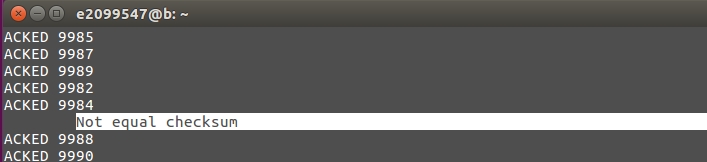
\includegraphics[width = \linewidth]{checksum.png}
\caption{Checksum in action}
\label{fig:checksum}
\end{figure}
\begin{verbatim}
	sendpacket = "PAYLOADHERE"
	sendpacket += "PACKETNUMBER"
	check = checksumfunction(sendpacket)
	sendpacket += check
	send(sendpacket)
\end{verbatim}
The same thing also happens in the destination 'd'. When it receives a packet, first it reads a 250 byte of it to extract information, next 6 byte to sequence number and last 16 byte to checksum. The destination 'd', then calculates message's checksum, again using MD5, and if both of them are equal and the sequence number is the expected one, it prepares a feedback and send back to the broker 'b'. \\
For detailed information about our previous implementation for the term project 2, please refer to the section at the end of this report.\\
\subsubsection{Pipelining}
The broker 'b' infinitely loops until it encounters an empty data, which is the final connection. 'b' calculates a size 'empty' which means how many packets that 'b' can receive in addition to its current buffer. In the beginning of the transmission, it is equal to the half of the window size. Thus, it receives 8 packets from 's', divides them into two and makes 16 packet to fill its window. When the buffer is full, it means it should not receive more packets.\\
After receiving all possible packets from 's', the buffer becomes full, so we cannot receive more data. The "file\_receiver" function waits until a condition happens, which is buffer is empty. If the buffer is empty condition is raised from other threads, which means that feedback receiver threads are received a feedback or the main thread wake up the sender thread for retransmission, the sender thread wakes up and tries to advance its window size by checking packets from start the end in its window range. If there are messages which are "ACK"ed, it can advance the window and begins to accept new packets from 's' again using 'empty' variable. Either it advances the window size or not, this thread check all packets in its window and tries to send them again if there is an error or timeout. It does not retransmit the messages that have a state of "ACK" and does not retransmit the messages that have a state of "SEND" and "RESENT" if they are send recently by looking at the timeout values.\\
Lastly, when there are no new packets coming from 's', this function loops in another infinite loop until the last elements in the buffer are sent and acked to make sure all the messages are sent correctly.\\
\subsection{Destination node 'd'}
In this node, like in the part 1, we have created two threads for UDP connection coming from routers. These threads are listening their connections to 'r1' and 'r2' separately and when the data comes, it looks the content of the packet. If the checksum inside the packet and the checksum of the data matches, it looks an additional info.\\ If the expected sequence number matches with the received sequence number it accepts the packet and prepares a packet which consists of received packet number, type "ACK" and a checksum. There might be a case, where the packet number 102 arrives before 100. In this case, destination 'd' will not accept 102, and the packet 102 will be resent. The other case is that, the destination expects a packet number with 102 but it received packet number 100. It means, it has previously received this number and to avoid infinite loop in 'b', it sends an "ACK" message of this packet.\\
If the checksum does not match, it does not anything and waits for retransmission. The timeout in the broker 'b' will retransmit. Then, it sends this feedback packet to the back where it comes from, 'b' over 'r1' or 'r2'. The broker will take an action by looking at the feedback packet's type.\\
\section{Routing tables}
\subsection{Broker b}
In the 'XML' file that we are given, the packets were going over the router 'r2'. We have looked at the routing table of the 'b' and saw that the destination '10.10.3.2' is connected to the gateway '10.10.4.2'. We have deleted this route and our current configuration is in the Fig ~\ref{fig:routeb}. For example, to configure routing table, we have used the following command:\\

sudo route add -net 10.10.3.0 netmask 255.255.255.0 gw 10.10.2.2 dev eth2\\

\begin{figure}[h!]
\centering
\captionsetup{justification=centering}
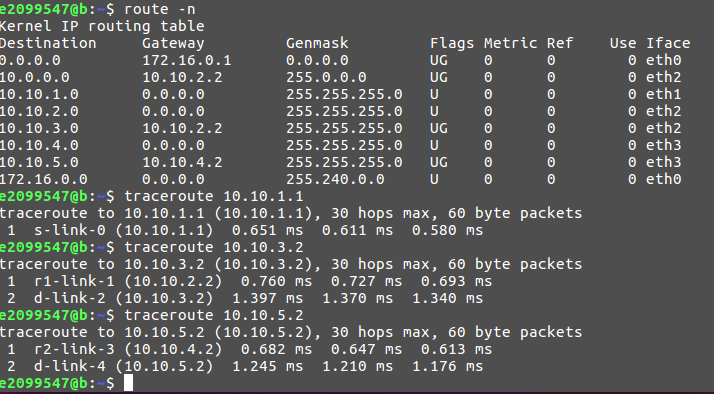
\includegraphics[width = \linewidth]{routeb.png}
\caption{Broker router table}
\label{fig:routeb}
\end{figure}
When the destination is '10.10.5.2' in broker, it should go over router 'r2'. Indeed, the netmask and gateway configuration of the table will allow us to forward the data to 'r2'.\\
We can clearly see that we have successfully configured routing tables in 'b', by running command 'traceroute IPADDRESS'. Packets with destination IP address '10.10.5.2' goes over 'r2', and packets with destination IP address '10.10.3.2' goes over 'r1'.\\
\subsection{Router r1 and r2}
\begin{figure}[h!]
\centering
\captionsetup{justification=centering}
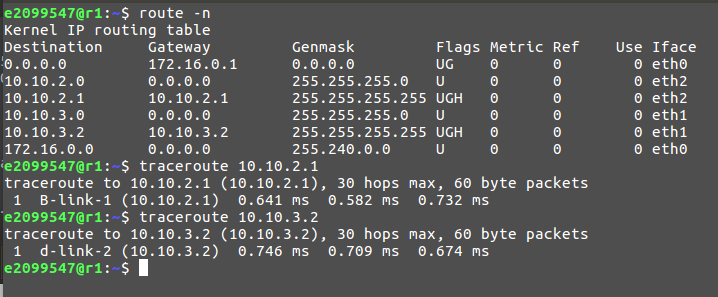
\includegraphics[width = \linewidth]{router1.png}
\caption{R1 router table}
\label{fig:router1}
\end{figure}
\begin{figure}[h!]
\centering
\captionsetup{justification=centering}
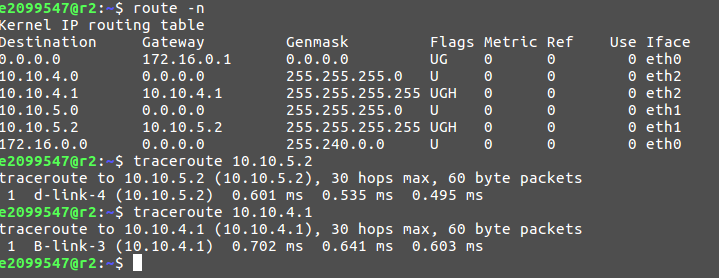
\includegraphics[width = \linewidth]{router2.png}
\caption{R2 router table}
\label{fig:router2}
\end{figure}
In this implementation, we don't run scripts in routers. We simply configured the routing table in these machines. They are forwarding the incoming data to correct output. If the data comes from the broker 'b', it is forwarded to 'd', if a feedback packet comes from 'd', it is forwarded to 'b'.
\subsection{Destination d}
\begin{figure}[h!]
\centering
\captionsetup{justification=centering}
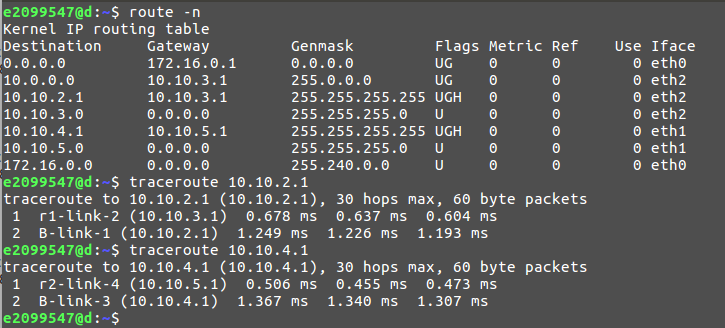
\includegraphics[width = \linewidth]{routed.png}
\caption{Destination router table}
\label{fig:routed}
\end{figure}
We have configured destination routing table such that, when a feedback packet goes to 'b', it goes over either 'r1' or 'r2'.\\
After the transmision is completed, we are writing the buffer into a file named "received.txt". When we run the file comparison function using python, we can see that the "input.txt" and "received.txt" are equal as in Fig ~\ref{fig:comparison}.
\begin{figure}[h!]
\centering
\captionsetup{justification=centering}
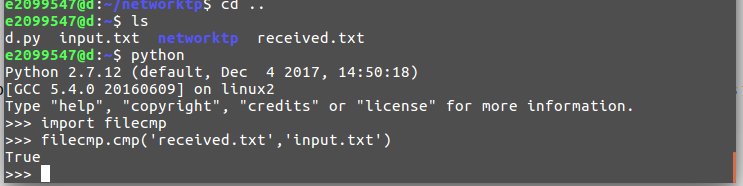
\includegraphics[width = \linewidth]{comparison.png}
\caption{Comparison of original and transmitted file}
\label{fig:comparison}
\end{figure}
\section{File Transfer Time Calculation}
We are calculating the file transfer time in broker 'b'. When packets come from the source 's', we are storing the current time of that packet.\\
When the file transmission is finished, meaning that we have sent all of the data and they are all "ACK"ed, the broker calculates difference between first packet's sent time and last packet's sent time. One can argue that, we should have used first packet's sent time and last packet's received time for measuring file transfer time. We have done this implementation in the first two version of this project and observed that there is not much difference between taking last packet's received time and last packet's sent time. Also, we have concluded that, the time field in the feedback packet adds additional cost to the network. Taking into account these observations, we did not measure received time in 'd', and send back to the broker 'b' as we did in the previous part of the project. Thus, we did not use time syncronization to the global time.\\
\section{Experiments}
In this project, we have conducted 3 different experiments. These are named loss, corrupt and reorder packet experiments. If we don't have any error in the interface (without applying the commands), on the average we are experiencing one or two duplicate packets and the file transfer time is 50 seconds.\\
In the broker 'b', it uses a similar method to selective repeat for retransmission. If the message is not acked, it waits for timeout of the packet, then it retransmits. In the destination 'd', it expects a desired sequence number and as it is explained before it takes an action when the sequence number matches or does not match with the expected one.\\
In these three experiments, we have applied given commands to both direction. For example, we added loss packet to b's interface connected to r1, and r1's interface connected to b.\\
At every 200ms, main thread in the broker 'b' wakes up the sender thread. The sender thread loops over the packets in the window and if their times are expired(in our case we did 500ms), it resends packets.\\
\subsection{Experiment 1 - Loss packet}
\begin{figure}[h!]
\centering
\captionsetup{justification=centering}
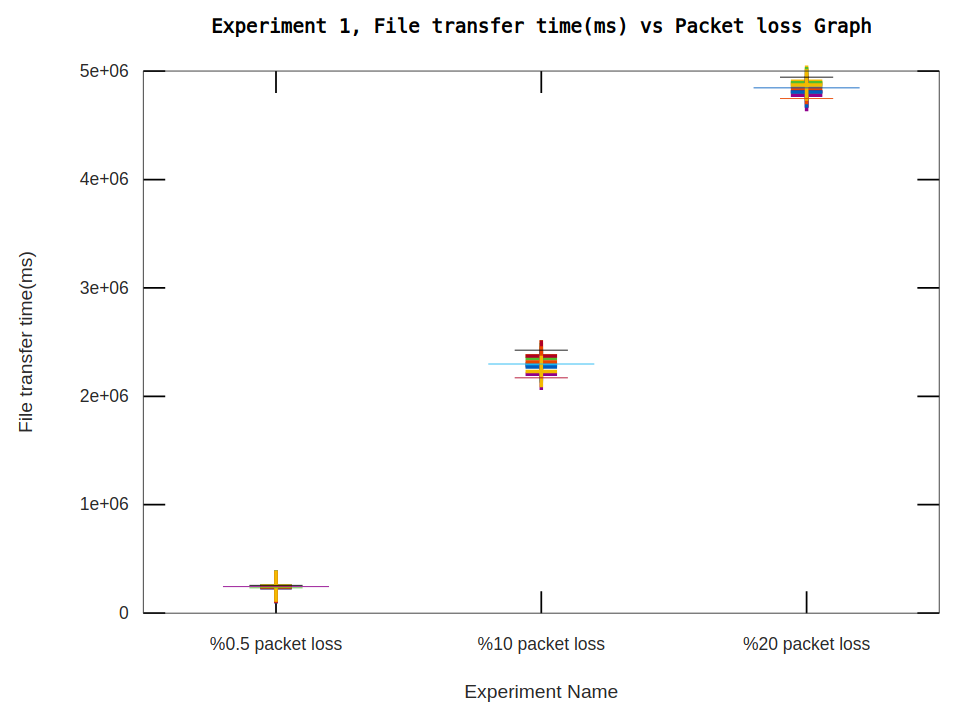
\includegraphics[width = \linewidth]{exp1.png}
\caption{Experiment 1 results}
\label{fig:exp1}
\end{figure}
The more loss rate, the worse our program runs. In the 3rd run, 20\% loss rate, one packet only arrives at the destination at a rate of 64\%. Its feedback packet also arrives at the same success rate to the broker 'b'. Thus, one successful attempt for a packet to be sent and acknowledgment is around 40\%.\\
Also, it is because, we have implemented a desired sequence number in destination 'd'. The previous implementations do not have this desired sequence number at destination 'd'. This desired sequence number slows our program massively if there are no corruption in the network. We added this feature to solve a situation, where the sequence number of the packet is corrupted but it is a still valid one and the checksum could not detect the error.\\
It is explained in detail in the next section, Conclusions and Remarks.\\
\subsection{Experiment 2 - Corrupt packet}
\begin{figure}[h!]
\centering
\captionsetup{justification=centering}
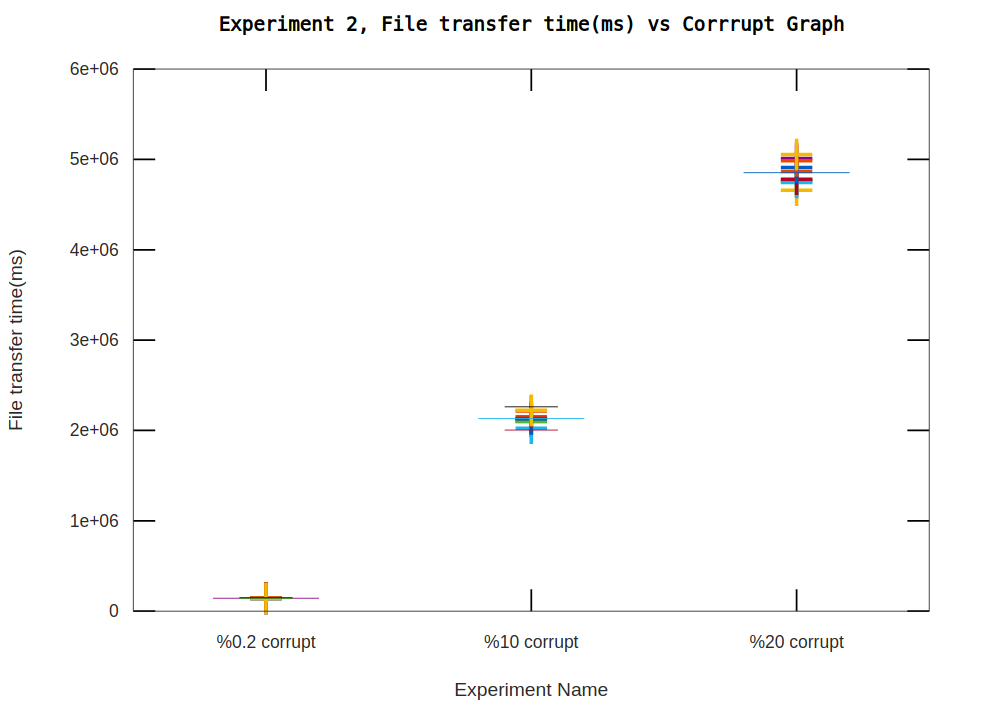
\includegraphics[width = \linewidth]{exp2.png}
\caption{Experiment 2 results}
\label{fig:exp2}
\end{figure}
The more corruption rate, the worse our program runs. The desired sequence number at 'd' allows us to transfer the file correctly at a high rate of corruption. However, it is massive drawback when it comes to the speed.
The worst case, which is 20\% corruption transfers our file nearly 100 times slower than the environment without a corruption.\\
Also, the first one, 0.2\% corruption case runs better than 0.5\% loss packet case. This is because of the expected sequence number at 'd'. If we did not implemented this, the first experiment could run much faster. However, since we employed this feature to cover all possible cases, the graphics are nearly the same. The only difference between first and second experiment is the first part of the data, 0.5\% loss and 0.2\% corruption. Packetloss experiment runs slower because the magnitude of the error is larger than the 2nd experiment.\\
\subsection{Experiment 3 -Reorder packet}
\begin{figure}[h!]
\centering
\captionsetup{justification=centering}
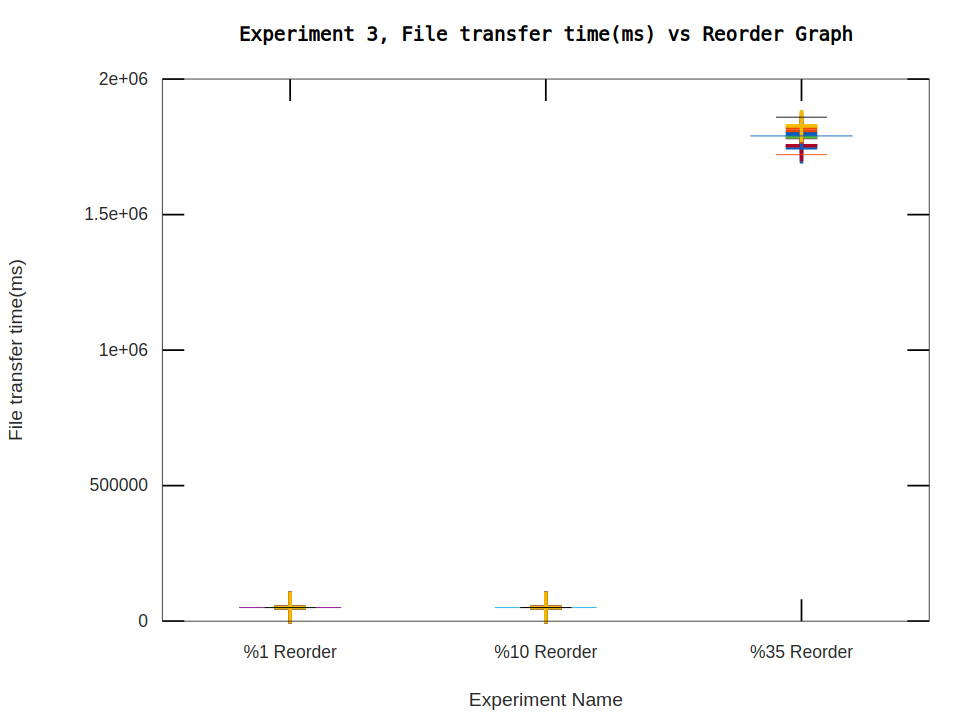
\includegraphics[width = \linewidth]{exp3.png}
\caption{Experiment 3 results}
\label{fig:exp2}
\end{figure}
Since our window size is small, 16, the reordering command does not affect our program in the first 2 sets of commands. We believe that, the 10\% reordering should have affected our program more, but it did not. Thus, we were probably lucky in those 10 experiments. However, if we do the reordering 35\%, it affects our program, but not so much as loss packets or corrupt packets. This is because, we are expecting a sequence number at the destination 'd'. If the packet's sequence number does not match with the desired number, it will be retransmitted later.\\
\section{Conclusion and Remarks}
We have improved our implementation three times throughout the project phase.\\
In both 3 version, we have tried the similar approach.
S reads the file sends to b if the b has empty in its window.
B packetize this into two parts, dividing from middle and sends to d through routers r1 and r2.\\
When the d receives it, it sends ACK, PACKET NUMBER to back.
B shifts its window appropriately and loops until file transmission is completed\\
We are putting all of our implementations in the submission folder, because we believe that it is best way to express our effort in this homework/project.\\
\subsection{Implementation 1}
In the version1, we have done the following parameters:\\
We read the file by decoding into 'hex'. This caused our file size to increase two times. When we read 200 bytes, converting it to hex results is 400 bytes.\\
After sending 400 bytes, b divides this into 2 parts. The payload of our data consists of 200bytes.\\
In B, we declare a dictionary, put the payload inside, then add the packet number. The checksum calculation is similar to TCP checksum calculation and we calculate checksum only the data, not including the packet number.\\
\begin{verbatim}
send data format:
	d['data'] = payload
	d['number'] sequence number
	d['checksum'] = checksum of payload
\end{verbatim}
After packetization, we send the data through routers, and the d will respond back in this format\\
\begin{verbatim}
	f['type'] = ACK or NACK
	f['number'] = seq# of recv packet
	f['time'] = recv time of packet
\end{verbatim}
We have observed that the send packet size is 256 byte and the received feedback packet size is 84 byte, which they add up to 340 byte. Since we have two links and both of them are 500kbits, in the full utilization we can send 128kb per second. We have specified the window size as 400 because 256 * 400 equals 102kbyte. The rest are reserved for feedback packets. Although, we believe that we can select a little less window size to achieve better results.\\
This implementation has bugs. These bugs are:\\
\textbf{1-} The payload size is 200 bytes. Our checksum function returns 5 bytes. This causes mapping to same position/number even if the data are different.\\
\textbf{2-} We did not protect the sequence number with checksum. In d, we have observed following patterns:\\
\textbf{a.} The sequence number is corrupted but still a number. However, it is previously ACKED. We simply ignore that issue and wait for retransmision. This was not a big problem.\\
\textbf{b.} The sequence number is corrupted and inserted in an empty position in the buffer of 'd'. Thus, incoming correct packet could not enter the buffer, because it was already data in there.\\
\textbf{c.} Everything received correctly in d. While sending feedback packet to b, since the feedback is not protected by checksum, the feedback packet corrupts. If the feedback packet's seqn corrupts and is still a valid number in the b buffer, it may accidentaly ACK not send or resent packets.\\
\subsection{Implementation 1.1}
In version 1.1, which we did not include in the submission folder, we have protected both payload and checksum number.\\
\begin{verbatim}
	data['data'] = payload
	data['number'] = seq#
	check = checksumfunction(data)
	data['checksum'] = check
\end{verbatim}
However, we still have this kind of situation\\
\begin{verbatim}
{u'checksum': u'00052076', 
u'data': u'06af12aa7997d8694a6ca8
d88d6f5927250df9648bc1790ccddddd0
b060bd5e0ca5d4b3a0dde08bb3e2b6c31
b0b9d150fce79cc461c45c2e291762529
4926657c2a4b463a0390c9f6a955af338
d5ff299c6b1da3e90334ca9ad244a210c
c0b93c06d641e', 
u'number': u'000150'}

{u'checksum': u'00052076',
u'data': u'46af12aa7997d8694a6ca8
d88d6f5927250df9648bc1790ccddddd0
b060bd5e0ca5d4b3a0dde08bb3e2b6c31
b0b9d150fce79cc461c45c2e291762129
4926657c2a4b463a0390c9f6a955af338
d5ff299c6b1da3e90334ca9ad244a210c
c0b93c06d641e', 
u'number': u'000150'}
\end{verbatim}
Where the data corrupts on the wire/interface. Sequence number did not change but the data changes. However, the checksum could not identify the error. First bytes of the two packets are different.\\
We have conducted runs on the experiments and 1/2 times in the 20\% corruption experiment, either we observed some empty space in the buffer of the 'd', or the buffer is full but because of the small capability of the checksum, the data is changed and file is transmitted incorrectly.
\subsection{Implementation 2}
Since the data payload is 200 bytes, the checksum could not fully detect the issue in the payload. We decreased payload to 20 byte, and added protection to both seq number and data, as in version 1.1\\
In this way, we can almost fully detect bit errors because the payload + seqn is relatively small to the previous implementations. However, due to decreased number of payload, packet number has increased. Morever, the send packet size is 76 bytes, the received feedback packet's size is 84 byte, and the payload is only 20 bytes. Experiments take much longer and we did not run all of the experiments because of the reasons above. We also added checksum to feedback packet.\\
\subsection{Implementation 3, Final version}
In version 3, which is the final version, we changed several stages of our implementation.\\
\textbf{1-} In s, instead of reading 20 bytes from file, then decode it in hex and forward it, we simply read all of the files line by line, then put it in a buffer string. After that we transmit 500 byte of this string at each request.\\
\textbf{2-} In b, instead of packetizing it in to a json object, or python dictionary, we append it to a string and added packet numbers etc to its tail.\\
\begin{verbatim}
	sendpacket = "PAYLOADHERE"
	sendpacket += "PACKETNUMBER"
	c = checksumfunction(sendpacket)
	sendpacket += c
\end{verbatim}
In the implementation above, the payload size is 250 byte per package, because we are dividing 500 incoming bytes into two.\\
Also we have changed our checksum function from TCP checksum to md5 for better accuracy.\\
\textbf{3-} As previous iterations, we added checksum to feedback function which is md5.\\
\textbf{4-} In the previous versions, not desired packet could enter the buffer. i.e., the packet 100 should have received, however it corrupts on its way. The checksum could not detect the error, and the received packets seqn is 105. We put this packet into buffer 105 and send back 105ACK message. When the 100 packet times out in b, it will be resent and and it will take its position in d buffer. However, the 105th packet in b already acked due to error. We don't retransmit this even though it is not correctly acked.\\
\textbf{5-} To avoid the issue above, the d now expects only one packet at a time. If the expected value is 100 and the received packet is 102, d does not accept this. It might have happened either because of the error in the network, or out of order. We don't care this situation, our top priority is reliability. If the expected value is 100 but we have received 98, we have correctly received this previously but we still send a 98 ack to back, to avoid infinite loop or stuck in b.\\
\subsection{Conclusion}
Our final implementation can successfully sends a file from a source to a destination. To detect errors, the TCP checksum is not sufficent enough for larger payloads. Using small payload with TCP checksum saves us from errors, however, due to the size of the payload is very small than the send packet size and the feedback size, the transmission time massively increases. Since the purpose of this homework is transferring a file reliably, we have implemented an expected sequence number check at the 'd'. This implementation affects performance if there are any kind of corruption or loss in our packets. However, the low amount of reordering packets did not affect our program so much, because our window size is small.
\end{document}



